\documentclass[a4paper]{article}
\usepackage[utf8]{inputenc}
\usepackage[margin=50pt]{geometry}
\usepackage{tabulary}
\usepackage{graphicx}

\title{Ingegneria del Software T}
\author{
    Luca Bartolomei 
    \texttt{0000825005}
    \\
    Luigi Di Nuzzo
    \texttt{0000824873}
    \\
    Filippo Veronesi
    \texttt{0000832244}
}

\date{Marzo 2020}

\begin{document}

\maketitle

\tableofcontents

\newpage

\section{Abstract}

Il progetto riguarda la creazione di un applicativo software gestionale per prevendite elettroniche.\\
Abbiamo pensato il software per un gruppo di amici che organizzano feste, con obiettivi cardine l'abbattimento di costi, l'ottimizzazione dell'entrata dei partecipanti all'evento e una semplificazione dei conti di bilancio.\\
L'idea di fondo è di utilizzare, come sostitutivo alla prevendita cartacea, un codice QR in grado di far entrare il cliente dopo relativo check all'entrata.\\
Il risparmio economico ottenuto è ovviamente importante in confronto alla vendita tradizionale. Tuttavia bisogna tenere in conto dei problemi tecnologici che si possono verificare durante la vendita e l'entrata: problemi di connessione Internet, incompatibilità dei dispositivi dei clienti, training del personale addetto alle entrate, eccetera.\\
Viene gestito oltre alle prevendite e relatvi clienti, anche l'organizzazione e i vari membri dell'organizzazione, con divisione dei ruoli.\\
Per facilitare i conti di bilancio è disponibile una sezione in cui è possibile ricavare statistiche sull'andamento dell'evento.

\section{Analisi dei requisiti}

\subsection{Requisiti del sistema}

\begin{itemize}
	
	\item \textbf{REQUISITI FUNZIONALI}
		
	\item Il software prevede la possibilità di gestire più staff.
	
	%-Requisiti di sicurezza
	
	%--Requisiti di identificazione
	\item Gli utenti devono essere identificati tramite username.
	
	%--Requisito di autenticazione
	\item Gli utenti sono autenticati tramite credenziali di username e password.
	\item L'accesso ad uno staff, da parte di un utente, avviene tramite codice di accesso.	

	%Funzionale/non funzionale
	\item La registrazione di utenti è a carico dell'amministratore di sistema.
	\item Possibilità di cambiare la password personale dell'utente.
		
	%--Requisiti di Autorizzazione
	\item Ogni membro di uno staff può ricoprire dei ruoli: cassiere, PR, amministratore.	
	\item Il ruolo di cassiere riguarda la timbratura di prevendite all'ingresso di un evento.
	\item Il ruolo di PR riguarda la vendita di prevendite a clienti.
	\item Il ruolo di amministratore riguarda la gestione dei membri, degli eventi, delle tipologie di prevendita di un evento e della visualizzazione di tutte statistiche.
	
	%--Requisiti di scoperta alle intrusioni
	\item Utilizzo di log per monitorare operazioni critiche.

	%--Requisiti di riservatezza
	\item Le password devono essere salvate in modo sicuro.
	
	%Non vuol dire cifrato! Basta un controllo agli accessi.
	%Se salvi in DB ricorda di indicizzare.
	%\item Il log deve essere salvato in modo abbastanza sicuro.
	
	%--------------------
	
	%Accesso e creazione di uno staff
	\item Ogni utente registrato nel gestionale può diventare membro di uno o più staff. 
	
	\item Quando un utente crea uno staff ne diventa membro e amministratore.
	
	%Timbratura (Cassiere)
	\item La timbratura di una prevendita valida permette al cliente di entrare all'evento, ovviamente lo staff potrà effettuare ulteriori controlli non previsti dal sistema e decidere di far entrare un cliente.
	
	
	%Non viene specificata la modalità di consegna: URL, file immagine file testo etc.
	\item La vendita di una prevendita elettronica consiste nella consegna al cliente di un documento digitale di qualche forma, associato alla prevendita elettronica venduta.

	
	%Gestione staff (Amministratore)
	\item Un amministratore può concedere/revocare i ruoli a qualsiasi membro dello staff. Unico vincolo è che rimanga almeno un amministratore.
	\item Possibilità di cambiare il codice di accesso dello staff da parte di un amministratore.
	   
	\item Per gestione degli eventi di uno staff si intende la possibilità di vedere gli staff di un evento, di creane uno nuovo e di poter modificare un evento dello staff.
		
	\item La gestione delle tipologie di prevedita di un evento indica l'aggiunta, la modifica e la rimozione delle tipologie di prevendita.
	
	%Definizioni
	%-Eventi
	\item Un evento è composto da un nome, una descrizione, un periodo temporale di svolgimento e un luogo. 
	\item Un evento può essere annullato, anche se ci sono prevendite vendute.
	
	%Tipologia Prevendita
	\item Una tipologia di prevendita serve ad associare alla prevendita un prezzo, una descrizione e un periodo di vendita a tutte le prevendite con la stessa tipologia.

	%-Prevendite
	\item Una prevendita può essere annullata e/o rimborsata. 
	
	%-Statistiche
	\item Le statistiche di un membro sono suddivise per ruolo coperto all'interno dello staff: cassiere o PR.
	
	%Si deduce dalla precedente
	%\item Il ruolo di amministratore non prevede statistiche personali.
		
    \item \textbf{REQUISITI NON FUNZIONALI}
	
	%Se si verifica attacco freezing dell'account cambiare username.
	\item Il blocco dell'account deve avvenire dopo 3 tentativi. Dopodiché l'amministratore di sistema deciderà se sbloccare l'utente.
	
	\item La password degli utenti deve essere lunga almeno 8 caratteri.
	\item Il codice di accesso allo staff deve essere lungo almeno 4 caratteri.
	\item Ogni utente registrato può creare al massimo uno staff.
	\item Requisito fondamentale è il basso costo del prodotto software.
	\item Utilizzare uno o più metodi per velocizzare l'autenticazione dell'utente.
	\item I membri non amministratori possono vedere solo le statistiche personali.	
	\item I membri non amministratori possono solo vedere le tipologie di prevendite associate ad un evento.
	\item I membri non amministratori possono solo vedere gli eventi dello staff.
	\item Il periodo di vendita delle prevendite deve essere antecedente il periodo dell'evento.
	\item Una prevendita annullata e/o rimborsata rimane tale.
	\item Un evento annullato rimane tale.
	\item Si prevedono più forme di consegna del documento digitale, per affrontare le eterogeneità.
	\item Il documento digitale consegnato al cliente sarà utilizzato dal cassiere all'ingresso timbrare la prevedita elettronica.
	\item La password fornita dall'amministratore di sistema a tempo di registrazione va cambiata immediatamente dopo il login.
	
	%Devo contare i tentativi falliti nel db: nella sessione potrei cancellare i cookie.
	\item Bloccare l'account utente dopo troppi tentativi di accesso e notificarlo nei log.
	
	\item Ogni ruolo è indipendente.
	\item Ogni staff gestito dal software è indipendente.
	
	%Utilizzo https per la cifratura
	\item Si richiede una comunicazione sicura.
	
	%Sistema locale senza server remoto tramite server locale + wifi
	\item Si richiedono procedure manuali o automatiche per cercare di garantire la disponibilità del servizio.
	
	%Codice della prevendita
	%Prevendita nominativa
	\item Si richiedono metodi per evitare la contraffazione delle prevendite.
	
	%Log
	\item Prevedere livelli di log per aiutare l'analisi da parte dell'amministratore di sistema.
	
	%Prevendita
	\item Ogni prevendita venduta è associata ad una sola tipologia di prevendita.
	\item Ogni prevedita è nominativa.
	
	%--Requisiti di non-ripudiabilità
	\item Quando un PR vende una prevendita, essa viene associata ad esso.
	\item Quando un Cassiere timbra una prevendita, essa viene associata ad esso.
	
	%Vendita (PR)
	\item Prima della vendita il cliente sceglierà una tipologia di prevendita associata all'evento a cui vuole partecipare.
	
	\item La timbratura può essere fatta solo una volta.
	
	
\end{itemize}

\newpage

\subsection{Analisi del dominio}

\subsubsection{Glossario}

\begin{table}[ht!]
  \begin{center}
    \begin{tabulary}{1\textwidth}{c|C|C}
        \textbf{Voce} & \textbf{Definizione} & \textbf{Sinonimi}\\
        \hline
        \hline
		Amministratore di sistema & Utente con privilegi di sistema aggiuntivi. & \\
		\hline
		Privilegio di sistema & Autorizzazione intrinseca concessa ad un amministratore di sistema che riguarda la gestione del software stesso. Non riguarda gli staff. & \\
		\hline
        Staff & Gruppo di utenti con lo scopo di organizzare eventi. & Ente organizzatore \\
        \hline
        Utente & Persona registrata nel software gestione. & \\
        \hline
		Cliente & Persona che vuole partecipare ad un evento di uno staff & \\
		\hline
        Membro & Utente che è iscritto ad uno staff. & Organizzatore \\
        \hline
		PR & Membro di uno staff che si occupa della vendita di prevendite & \\
		\hline
		Cassiere & Membro di uno staff che si occupa dell'entrata dei clienti ad un evento & \\
		\hline
		Amministratore & Membro di uno staff che si occupa della gestione dello staff steso & \\
		\hline
        Ruolo & Autorizzazione che ha il membro all'interno dello staff & Autorizzazione \\
        \hline
        Evento & Avvenimento registrato dallo staff, per il quale è possibile vendere prevendite e registrare ingressi & Festa \\
        \hline
        Tipologia Prevendita & Modello associato ad un evento, la quale da le caratteristiche di prezzo e descrizione alla prevendita venduta & Tipo Prevendita \\
        \hline
        Prevendita & Biglietto venduto anticipatamente, che consente l'entrata all'evento pagato & Ticket, Prevendita Elettronica \\
        \hline
		Statistiche & Informazioni di carattere gestionale, riguardo ad un evento o a un membro dello staff & \\
		\hline
		Documento digitale & Si tratta di una risorsa digitale, reperibile dal cliente, che serve a identificare una prevendita venduta & \\
		\hline
		Log & Registro dove vengono salvate informazioni per risalire ad operazioni critiche svolte & Registro \\
		\hline
		Operazione & Comando richiesto al software gestionale da parte di un utente & \\
		\hline
		Login & Operazione per identificare un utente & Accesso utente \\
		\hline
		Timbratura & Operazione svolta da un cassiere svolta per validare una prevendita di un cliente & Convalida della prevendita \\
		\hline
		Credenziali & Coppia di valori username e password utilizzata per l'autenticazione dell'utente & \\
		\hline
		Username & Stringa di caratteri alfanumerici. Serve a identificare l'utente & \\
		\hline
		Password & String di caratteri alfanumerici. Può contenere caratteri speciali. & \\
		\hline
		Periodo di vendita & Periodo temporale in cui la prevendita è vendibile ai clienti & \\
		\hline
    \end{tabulary}
  \end{center}
\end{table}

\newpage

\subsection{Casi d'uso}

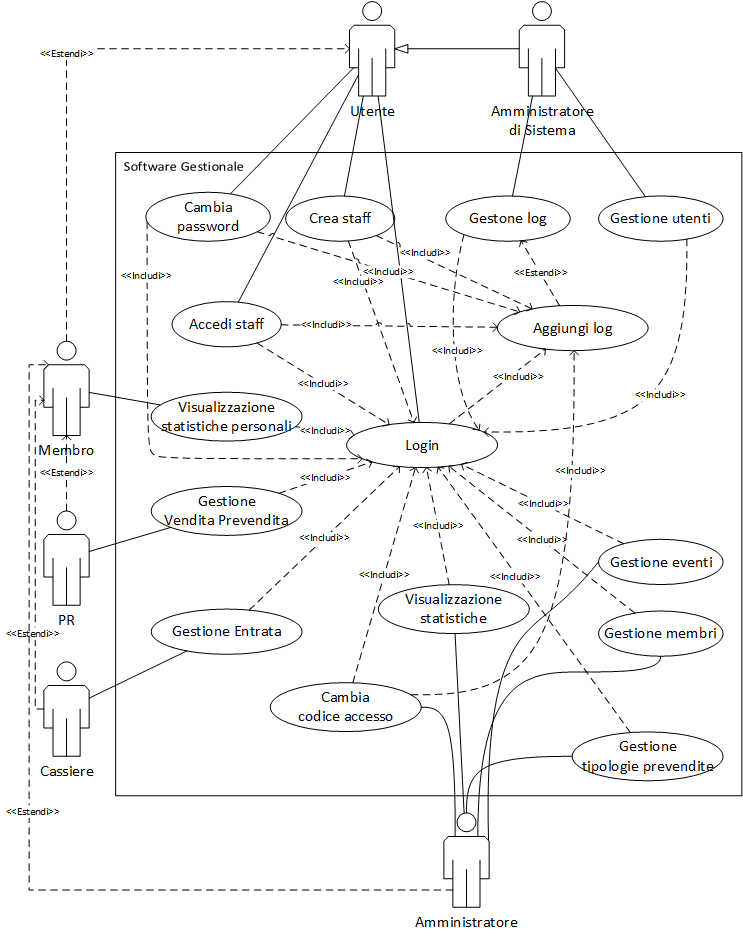
\includegraphics[scale=0.9]{use_cases.png}

L'utilizzo del login è necessario per tutti i servizi forniti agli attori.
Non abbiamo approfondito molo in quanto si avrebbe avuto un diagramma pesante per la lettura.
Tutte le funzioni che abbiamo ritenute critiche utilizzano il caso d'uso "Aggiungi log".
Abbiamo differenziato i casi d'uso delle statistiche perché si tratta di concetti diversi.



\subsection{Scenari}

\end{document}
